\documentclass[10pt]{article}
\usepackage{amsmath,amssymb,booktabs,hyperref,placeins}
\usepackage{style/hkustgz-paper}
\hypersetup{pdftitle={Design Success and Method Evidence: Controlled Transfer in Battery-Free Design},pdfauthor={Working draft}}
\title{Design Success and Method Evidence:\\Controlled Transfer in Battery-Free Design}
\author{Working draft}
\date{20 October 2026}
\begin{document}
\maketitle
\begin{abstract}
A successful design does not by itself validate its design method. We study this
distinction in a fixed executable battery-free apparatus, separating device
programs $D$, design procedures $H$, and procedures $G$ that generate $H$.
Global method changes require fresh decisions, while input-identical lower-level
responses may be reused. An early recovered method produces a passing device but
fails independent promotion. A prospective comparison then gives 12/12 service
passes to every method, with 64 requests for fixed $H_0$, 117 for ordinary
reflection, and 127 for the typed procedure. We next form two actual
model-authored timing methods from the same retained failure history and freeze
them before new task execution. Across three timing conditions and two fresh
contexts, fixed $H_0$, $H_0$ with the same history, ordinary reflection, and the
proposed method each pass 6/6, using 28, 26, 43, and 29 formal requests.
The proposed method adds no success, request, or charge advantage over the
equal-history baseline. Frozen relations return false on six successful ordinary
designs and two successful proposed designs; these returns require scope-aware
interpretation, rather than equating design success with method proof. Formation,
validation, first use, and final execution costs remain separate. Earlier
improver-lineage differences, four token-censored attempts, and A/R product
failures remain in the record. These finite digital results establish neither
general method superiority, recursive self-improvement, nor physical acceptance.
\end{abstract}
\section{Introduction}
An agent can change a device, change how it designs devices, or change how it
proposes future design methods. These interventions have different evidence
requirements. A new capacitor must be checked against the coupled controller
response. A new design method must make fresh decisions on a fixed task. A
successful descendant method does not establish that its proposer reliably
improves. Confusing these objects can turn valid local execution into an
unsupported claim of general scientific progress.

Battery-free systems make these distinctions observable. Harvested input,
storage voltage, boot timing, sensing and transmission constrain one another.
A reset after delivery need not destroy service, whereas a reset with pending
volatile state can. Retaining old records does not establish continued sensing
in darkness. Likewise, correct event detection and prompt reception can still
carry an inaccurate timestamp. The application contract and the actual temporal
record must decide acceptance independently of the agent's explanation.

We use a fixed executable apparatus with source-bound tools and an external
evaluator. The participant may change a legal artifact; it cannot change the
service or declare its own final acceptance. We distinguish device programs
$D$, design procedures $H$, and proposers $G$ that generate $H$. After a global
method change, we restart decisions at task entry, while permitting exact-input
reuse of qualified lower-level responses. This is a conservative validity
policy, not a claim of faster coupled simulation.

The experiments expose three obstacles to a method-improvement claim. An early
recovered model-authored method produces a passing design but fails independent
promotion because cache parity is missing and its necessary constraints exclude
a passing control. A subsequent prospective comparison matches initial caches:
fixed $H_0$, ordinary reflection and a typed procedure all pass 12/12 groups,
with 64, 117 and 127 requests. The later exploratory $G$ study produces descriptive
7/9, 6/9 and 8/9 transfer counts, conditional on one shared formation, and retains
four output-censored attempts. These results motivate an explicit test of
whether a frozen relation learned from original failures transfers beyond
unchanged $H_0$ given the same history.

The new C24 study answers that narrower question. Two actual model-authored
methods are formed once, validated separately and frozen before three new timing
conditions. All four arms---task-only $H_0$, equal-history $H_0$, ordinary reflection
and the proposed method---pass 6/6. The proposed arm uses more requests and a
higher charge estimate than equal-history $H_0$. Its relation returns also
expose a domain boundary that passing designs alone cannot resolve. We preserve
the earlier negative results, all original failures, formation and validation
costs, and the A/R product's independent service failures.

The contribution is an experimental validity contract and its measured limits:
separation of $D/H/G$ evidence; a negative prospective method comparison; a
frozen equal-history transfer test with independent service and relation checks;
and an auditable accounting of the earlier improver lineages. No general prompt
optimizer superiority, stable recursive self-improvement or physical device
acceptance is established.

\section{Experimental objects and validity contract}
Let $W$ denote the fixed world, $T$ the task and service contract, $D$ the device
program, and $E$ the external evaluator. The complete response
$Y=F(W,T,D)$ contains the coupled physical and controller trajectory, and
$E(T,D,Y)$ produces the computational service result. A design procedure $H$
chooses observations, orders experiments, and produces $D$ from a fresh task
entry. A proposer $G$ reads an admitted development history and generates
candidate $H$ artifacts for a registered selection procedure. The device's
runtime, an agent's decision span, and successive method generations are
different experimental axes.

The experimental dependency is $G\rightarrow H\rightarrow D\rightarrow Y$.
The arrows transfer an artifact or response, never an acceptance verdict.
Task, world, evaluator and budget authority remain external.


For a changed $D$, a reusable record must match all consumed inputs, apparatus
identities, numerical settings, and output bindings. The old trajectory is an
explicit negative control when a coupled input changes. Dependency and
boundary/scope invalidation may conservatively expand to the complete feedback
response. An exact-input cache can reuse a qualified response; building that
cache still has a cost. An evaluator-only change may reuse the same raw response
while requiring a new verdict. It cannot silently replace the previous verdict.

For a global $H\rightarrow H'$ change, our conservative policy restarts decisions
at task entry with a new owner and empty decision context. It does not replay
the old agent's reasoning as evidence for $H'$. Qualified lower-level responses
may still be reused when their consumed inputs match. A smaller restored decision
suffix would need its own state-validity proof; no such advantage is reported
here. A $G$ comparison additionally fixes $H_0$, the allowed development history,
selection tasks, future-input exclusion, and total improvement budget. Every
candidate branch, including an unselected sibling, remains part of that cost.

Promotion is a separate decision from schema eligibility and service success.
The method artifact records a hypothesis, falsifier, typed change and scope.
The external registry checks source, tool, model configuration, evaluator,
initial cache, fresh-context and cost identities. A structural pass admits an
artifact for testing; it does not validate the artifact's scientific claims.
The default method changes only under the registered retention rule.

\section{Apparatus, tasks, and measurements}
The principal apparatus is an ideal digital battery-free model with piecewise
source input, finite storage, conversion and sleep costs, boot and loaded-voltage
thresholds, event capture, and a receiving endpoint. In the small BF tasks, legal
device edits are capacitance and the earliest allowed transmit time. Event,
source, initial state, all other device fields and evaluator stay fixed. The
service requires the specified application frame by its deadline without
duplicate acceptance. Independent consumers check energy, receiver behavior,
transient voltage and deduplication. Passing these computations is not physical
calibration or an official benchmark result.

The prospective method comparison uses four fixed task IDs: fast-pulse BF,
volatile-reset BF, latched-reset BF, and a synthetic C-Lite single-query DC
derivative. They exercise distinct mechanisms within a small declared model,
not four independent hardware families. The C-Lite case does not qualify RF,
nonce security, multiple-query operation, or a real radio deployment. The formal
task list is finite; repeated sampling on a task is not an additional task.

The continuous A/R case concerns an indoor-light-powered temperature/history tag.
It couples photovoltaic port power, a capacitor, regulator thresholds, sensing,
persistent writes, record ranking, transmission and a digital gateway. Source
power is specified in watts; illuminance is descriptive metadata. The legal
apparatus starts with no stored energy and has an uncalibrated source, storage
and write model. It provides an engineering counterexample to broad completion
claims, not a physical demonstration. Section~\ref{sec:ar} preserves that case's
separate service and ordering requirements.

We measure independently evaluated service, participant service judgment,
ordered capture--reset--delivery events, admitted response identities, provider
requests, token-based charge estimates, summed episode wall time, failed actions,
resource censoring, native dispatch and new scientific execution. Requests,
logical design checks, cached response files and physical experiments are not
interchangeable counts. Public feedback is available to the participant; the
external final verdict remains separate. Developer assistance, model-weight
identity and physical qualification have their own boundaries.

The new C component in Section~\ref{sec:c24} isolates timing under continuous
power. Its complete service has three gates: event matching, timely reception,
and timestamp accuracy. The earlier O waveform service, this time component,
and the continuous A/R product are different contracts. We never pool their
PASS counts into a product-completion score.

\section{Earlier prospective comparison: a saturated strong baseline}
\subsection{Conditions, parity, and frozen sampling}
After the rejected confirmation in Appendix~\ref{sec:early}, the prospective protocol compares three method conditions under complete-raw information:
fixed $H_0$, ordinary reflection, and a typed dependency/evidence-scope procedure.
Complete-raw supplies all declared sources and the fixed model definition;
the host retains full raw traces for audit. Ordinary reflection reviews the
provided observations and proposes a method or no update. The typed procedure
additionally requests a $D/H$ distinction, source-dependent evidence scope,
event ordering, and separation of necessary constraints from sufficient
heuristics. It supplies no winning device values. Both proposing conditions
must produce actual model-authored hypothesis, falsifier and method text.

Each task/condition/repetition group has the same total cap of 24 requests,
1,200 seconds and two distinct $D$ candidates. The proposal subcap of eight
requests and 400 seconds is included, leaving less for fresh design when it
is used. Acquisition, failed actions, proposals, no-update decisions, fresh
design and confirmation are charged. Equal ceilings do not imply equal
realized spending. A no-update retains its cost and uses the base method for
an admitted fresh design.

Every arm starts from the same immutable cache manifest of 12 prior responses
plus one registered derived baseline. Job overlays are isolated. Later exact-input
deduplication does not expose another arm's output before its query or increase
the logical two-design allowance. All 28 matched proposal groups, including
pilots, pass the recorded information, tool, model-alias, cache and total-budget
parity checks. These are eligibility checks, not evidence of benefit.

Two pilot repetitions reverse condition order. The registered rule selects two
formal repetitions only if service and design signatures are stable in every
matched arm; otherwise it selects three. The pilot signatures are not stable,
so three repetitions are frozen once before formal execution. No original
failure is replaced and no outcome-dependent extension follows that freeze.
The complete eight-condition matrix has 16 pilot and 96 formal groups, comprising
140 episodes and 771 requests. The method subset uses six pilot and 36 formal
groups within that matrix. Its fixed-method cell is shared with the interface
study and counted once.

\subsection{Service ties and a negative retention result}
\begin{table}[htbp]
\centering\small
\begin{tabular}{@{}lrrrr@{}}
\toprule
Method & PASS/groups & Requests & Updates & USD upper \\
\midrule
Fixed $H_0$ & 12/12 & 64 & --- & 0.4231806 \\
Ordinary reflection & 12/12 & 117 & 10 & 0.8190117 \\
Typed procedure & 12/12 & 127 & 12 & 0.9367914 \\
\bottomrule
\end{tabular}
\caption{Fresh method comparison on four fixed digital tasks times three repetitions. All proposal and fresh-design requests are included. The base cell is shared with the interface matrix and counted once.}\label{tab:methods}
\end{table}

Each method passes all 12 formal groups, with task-success vector $(3,3,3,3)$.
Ordinary reflection proposes ten updates and returns no-update twice; the typed
procedure proposes in all twelve. Their total requests are 117 and 127 versus
64 for fixed $H_0$, including proposal and fresh design. The respective means
are 9.750, 10.583 and 5.333 requests per group. All no-update costs remain.
Different intermediate reasoning or device choices add no complete-service
success to this saturated baseline.

The registered rule requires strictly more task-level service success than
both controls, no lost task, and no higher mean request count. The proposed
procedure meets neither the strict success improvement nor the request criterion.
The selection therefore keeps the unchanged base $H$. This is a negative
result on the registered objective, not a claim that reflection can never help.
Four public digital tasks and repeated sampling do not estimate performance
over a broad population of products. The $H$ artifacts are instantiated locally
per group; no single global $H$ was transported unchanged across these tasks.

The full matrix costs USD 5.4478605 upper: 112 pilot requests at USD 0.7345845
and 659 formal requests at USD 4.7132760. All 771 settle. The 308 requests in
the main formal method subset already belong to that total and are not charged
again as a separate campaign.

\subsection{Correct recomputation without local savings}
The response audit annotates 107 existing admitted group responses; five groups
have no admitted final response. Of those 107, 91 change $D$ and 16 are unchanged
controls. A frozen old trajectory is ineligible after a changed coupled input.
Dependency, scope and full-feedback strategies share one actual complete-response
execution key in every admitted record. The first two conservatively expand to
full response, demonstrating no valid smaller suffix or speed advantage. For
a global $H$ change, all valid policies require fresh task-entry decisions.
This deterministic audit adds zero scientific execution and is not four new
paid strategy arms.

Four formal groups choose a pending event delivered across reset: two fixed
method groups, one typed-procedure group and one table-interface group. All
reuse the same historical latched-reset response at $10\,\mu$F / $45$ ms:
capture at 3.7--7.9 ms, brownout at 12.1 ms, and reception of the same event at
46.9 ms. Four fresh choices therefore represent one historical ideal response,
not four physical experiments or a newly invented memory mechanism. The other
83 successful formal groups deliver before any reset. Physical qualification
remains UNKNOWN in every case.

\section{Controlled transfer from the same failure history}
\label{sec:c24}
The earlier comparison re-formed a local method within each task group. It did
not test a single frozen method transported to new timing mechanisms. The older
waveform study also left a concrete ambiguity: successful designs used a
0.75 s sampling period, but a fixed-method control did so as well
(Appendix~\ref{sec:lineages}). Remembering that value cannot establish a general
relation among sampling, confirmation, timestamp origin and allowed error.
C24 therefore tests frozen method transfer with an explicit equal-history
control. Its prespecified falsifier is no gain against that control; the observed
result meets this falsifier for an improvement claim.

\subsection{A timing component with independently checked service}
This new component intentionally isolates time semantics under ideal continuous
power and a fixed link delay. It does not rerun or qualify the original O
energy, RF or keepalive service. The fixed waveform defines continuous threshold
excursions. An event qualifies only after its required confirmation duration;
the task then defines its true timestamp as either excursion onset or
qualification time. At each scheduled poll, the program first confirms the
previously held observation and then applies the new sample. The program never
reads the reference event list or acceptance verdict.

Legal $D$ fields are sampling period, sampling phase, timestamp origin, and a
constant timestamp offset. Origins are the confirmation poll, first qualifying
sample, or the midpoint between that sample and its preceding scheduled sample.
The fixed clock law applies signed constant drift, followed by nearest-grid
timestamp rounding and the existing millisecond frame encoding. Reception is
detection time plus the fixed 70 ms link delay. Event matching, timely reception,
and timestamp accuracy are independently checked; passing only one gate is not
complete service. In particular, timely delivery can carry a wrong event time.

\begin{table}[htbp]
\centering\small
\begin{tabular}{@{}llrrrr@{}}
\toprule
Task & Event time & Start/stop confirm. (s) & Quantum (ms) & Tolerance (ms) & Clock (ppm) \\
\midrule
Phase & Qualification & 3.00 / 4.00 & 20 & 130 & $+150$ \\
Confirmation & Qualification & 1.37 / 2.83 & 80 & 180 & $-250$ \\
Definition & Onset & 1.90 / 3.10 & 200 & 160 & $+300$ \\
\bottomrule
\end{tabular}
\caption{The three frozen formal timing conditions. Waveform transitions are
off-grid; the task JSON also fixes the source waveform and 6.5 s matching and
delivery windows. These are three within-model task conditions, not independent
hardware families.}\label{tab:ctasks}
\end{table}

\subsection{Formation, freezing, and exposure controls}
The four arms are unchanged $H_0$ with the task and public apparatus; unchanged
$H_0$ plus the original failure history; ordinary reflection from that history;
and the proposed typed timing procedure from the same history. The last three
receive identical historical information and source/tool permissions. Ordinary
reflection has access to the same executable relation language as the proposed
arm. Thus the comparison does not give one learned method an interpreter that
its control lacks. The task facts and legal design tools are common to all four.

Each reflection arm has exactly one actual model-authored formation and one
independent validation episode. Formation sees the retained original O failures,
not the new validation, first-use or final task inputs. Codex supplies task
mechanisms, a generic expression interpreter and independent evaluation; it does
not supply the learned equation. A method submission contains hypothesis,
falsifier, method text and up to eight named Boolean expression trees. The
interpreter permits fixed arithmetic, comparison and logic operators with
declared timing variables; it accepts no executable source code. Structural
admission means this artifact can be consumed, not that its claims are true.

Both structurally admitted original methods are frozen and carried unchanged
through validation and final use, including false relation returns. Validation
does not select the better method or authorize rewriting a failed clause. The
proposed arm also receives one separately identified first-use task; that result
is excluded from the final 24-attempt denominator. No new method is formed from
that success. There is one $H$ formation per reflection arm, not six independent
formations or a new $G$ lineage experiment.

The finite final list is three conditions times four arms times two fresh
contexts. Each solver entry permits at most 12 model requests, 900 s, 40 tool
calls and two distinct designs, with no automatic retry. Ordinary and proposed
formation use the same admitted limits and one-submission rule. The common
65,536-token output ceiling was frozen before the new batch. It does not replace
or reclassify the four older 32,768-token-censored attempts.

The sealed input audit checks 48 actual initial API payloads and 129 bound source
files across ABC, verifies within-task input parity and the shared history's
semantic identity, and reports only the model alias \texttt{deepseek-flash}.
Underlying model weights/version remain UNKNOWN. C-specific final references
bind all 24 episode-result byte hashes and both original method files. These
saved-data checks add no model request or scientific execution.

\subsection{The learned relations are hypotheses with a domain}
The ordinary method proposes a centered sampling budget that adds half a sample
period, half the timestamp quantum, definition delay, clock-error bound and link
delay. It also prescribes an origin-dependent offset. The proposed method
separates confirmation-grid alignment, origin/clock/rounding error,
sub-confirmation excursions, and delivery delay. In its qualified-event domain,
its origin budget has the form
\begin{equation}
 B_H=\frac{p}{2}+|\delta-c(o)|+e_{\rm clock}+\frac{q}{2}
 \;\leq\;\epsilon,
 \label{eq:learned}
\end{equation}
where $p$ is sample period, $\delta$ the offset, $o$ the timestamp origin,
$q$ the quantum and $\epsilon$ the task tolerance. Its stated centers are
$c(\mathrm{detected})=-p/2$, $c(\mathrm{midpoint})=0$, and
$c(\mathrm{first})=C-p/2$, where $C$ is confirmation duration. Equation~\ref{eq:learned}
reports the frozen model hypothesis, not a theorem established by this study.
The proposed artifact explicitly requires qualification-time semantics; the
onset task can therefore lie outside this relation's asserted domain.

The proposed sub-confirmation check instantiates the largest short excursion as
$d_{\rm short}=0.75C$, inherited from the original history. That ratio is not a
universal law of future waveforms. A syntactically general variable expression
can retain a history-specific premise. Neither artifact is hand-edited to make
its relations agree with final outcomes.

\subsection{All four arms succeed; the equal-history control is cheaper}
\begin{table}[htbp]
\centering\small
\begin{tabular}{@{}lrrrr@{}}
\toprule
Arm & Service PASS & Requests & USD upper & $H$ false on PASS \\
\midrule
Fixed $H_0$ & 6/6 & 28 & 0.1815672 & --- \\
$H_0$ + history & 6/6 & 26 & 0.6988500 & --- \\
Ordinary reflection & 6/6 & 43 & 1.1057187 & 6/6 \\
Proposed method & 6/6 & 29 & 0.7532616 & 2/6 \\
\bottomrule
\end{tabular}
\caption{C24 formal transfer: three task conditions times two fresh contexts per arm. Every design passes event matching, timely reception and timestamp accuracy. The last column counts successful designs with at least one frozen relation returning false; it is not an error rate or a proof of unsoundness. The fixed controls submit no learned relation set. Costs here exclude the separately listed formation, validation and first-use stages.}\label{tab:cformal}
\end{table}

All 24 submitted final designs pass every time-component gate, with no wrong
service judgment, incomplete entry or token-censored entry in this new list.
The proposed arm uses 29 requests and USD 0.7532616 upper, versus 26 and
USD 0.6988500 for unchanged $H_0$ with the same history. It therefore adds no
success and uses three more requests and USD 0.0544116 more even before charging
formation and validation. Ordinary reflection uses 43 requests and
USD 1.1057187. The task-only $H_0$ also succeeds 6/6, at 28 requests and
USD 0.1815672. History exposure and token length make this last comparison
different from the equal-history contrast; request count and token charge are
separate cost measures.

\begin{figure}[htbp]
\centering
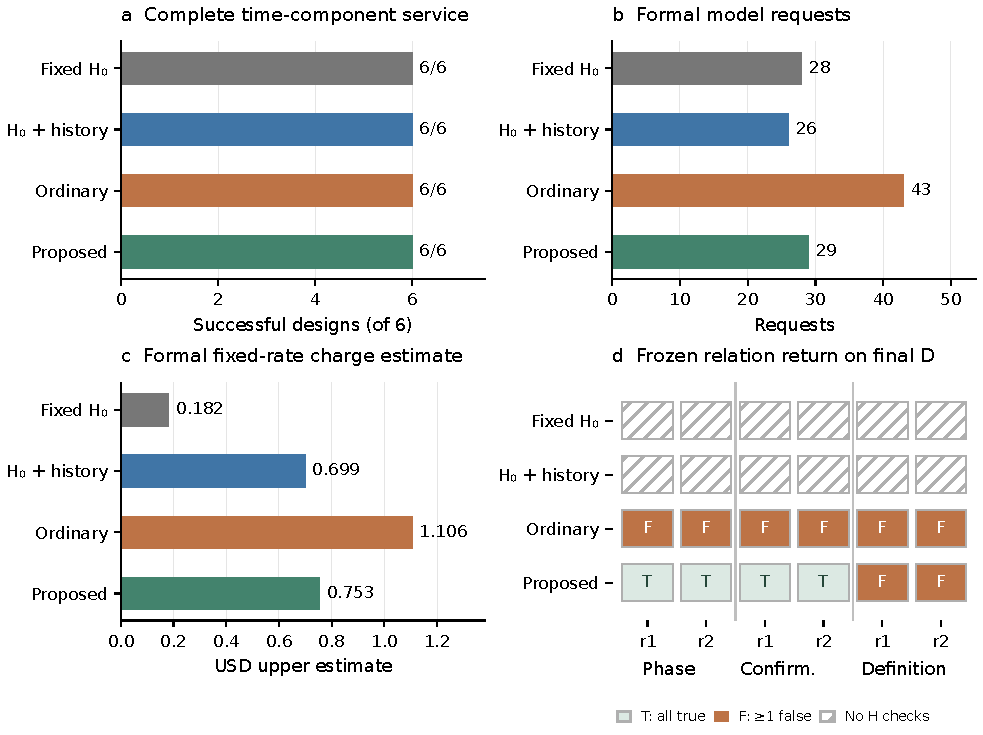
\includegraphics[width=\linewidth]{figures/c24-evidence.pdf}
\caption{The C24 result has three distinct evidence axes. (a) Every arm passes
6/6 complete timing services. (b,c) Formal requests and upper charge estimates
give no proposed-method advantage over equal-history $H_0$. (d) T means every
executed frozen relation returns true on that final design; F means at least
one returns false. Hatched controls submit no learned relation set. All cells
in (d) still have service PASS. These are exact finite observations, with one
method formation per reflection arm; no confidence intervals or population
claim are implied. False relations may flag scope or conservative constraints
and are not automatically scientific errors.}\label{fig:c24}
\end{figure}

\begin{table}[htbp]
\centering\small
\begin{tabular}{@{}lrrl@{}}
\toprule
Stage & Requests & USD upper & Independent result \\
\midrule
Ordinary formation & 4 & 0.1072422 & Structural admission \\
Proposed formation & 6 & 0.1660608 & Structural admission \\
Ordinary validation & 7 & 0.1832448 & Design PASS \\
Proposed validation & 5 & 0.1389699 & Design PASS \\
Proposed first use & 5 & 0.1198866 & Design PASS \\
\midrule
Formal transfer only & 126 & 2.7393975 & 24/24 design PASS \\
All 29 C episodes & 153 & 3.4548018 & No missing usage \\
\bottomrule
\end{tabular}
\caption{C learning and execution costs, charged once per actual episode. Both methods are carried unchanged into final use; validation is not an outcome-based selection gate. The first-use episode belongs only to the proposed arm and is excluded from C24. USD values use frozen token rates and are not invoices.}\label{tab:cstages}
\end{table}

The formal batch uses 126 requests and USD 2.7393975. Adding the two formations,
two validations and proposed first use gives 29 actual C episodes, 153 requests
and USD 3.4548018. All linked provider rows settle. The formal entries record
30 digital scientific executions and no exact-input cache reuse; these counts
are distinct from 126 model requests and 24 final designs. Formation has zero
scientific design execution. This saved-data paper preparation adds none.

\subsection{Why successful designs do not settle the methods' semantics}
Six of six ordinary final designs and two of six proposed final designs have
at least one frozen relation returning false (Figure~\ref{fig:c24}d). This is
a report of the original relations, not an automatic count of unsound methods.
A sufficient condition may reject a feasible design, and a domain guard may
correctly reject a task outside its assumptions. An independent design PASS
therefore neither proves the method nor, by itself, disproves every failed
relation. The artifact's prose and falsifier must also be read against its
declared direction of implication and domain.

For ordinary phase-r1, the design uses a 20 ms period, zero phase,
confirmation-poll origin and $-10$ ms offset. It passes all three service gates,
yet \texttt{centered\_sampling\_budget} and
\texttt{offset\_matches\_centering} return false for both event kinds. The
same two checks return false in confirmation-r1, despite design success.
The frozen qualified-event confirmation/offset prescription is not satisfied
by these participant designs. That discrepancy remains visible; success does
not overwrite the relation returns or establish the prescription's necessity.

For proposed definition-r1, $D$ uses an 80 ms period, 60 ms phase,
\texttt{first\_sample} origin and $-40$ ms offset. Event matching, timely
reception and timestamp accuracy all pass. Nevertheless,
\nolinkurl{event_time_definition_is_qualification} and
\nolinkurl{origin_clock_quantum_budget_within_tolerance} return false on
both start and stop. The task defines event time as onset, so the first false
may be a legitimate scope warning. In definition-r2, only that guard is false.
These results do not confirm transfer of all qualified-event clauses to onset
semantics. They demonstrate successful design execution alongside an unresolved
method-domain boundary.

The study has no independent repeated $H$ formations, clause ablation,
significance test or new hardware family. The three task conditions are finite
and every baseline succeeds, limiting sensitivity to a method gain. The
appropriate outcome is a negative improvement result on this registered
comparison, accompanied by an explicit record of what the frozen relations
did and did not accept. No $G$ expansion or recursive self-improvement follows.


\section{The product boundary remains independently negative}
\label{sec:ar}
The A/R tag provides a separate continuous device-level case. Its retained
reference has 348 samples on a six-hour profile and first fresh reception at
773 s. In a twelve-hour dark history profile it retains all 170 records,
including 168 whole-profile temperature samples, yet 648 of 720 historical
dark-window bins contain no new sample. All 73 backlog records miss the
recovery deadline and one of two required temperature events is missed.
In gateway recovery, all 60 queued records are acknowledged within 82 s and
duplicate arrivals cause no duplicate acceptance, but one fresh sample waits
30 s. Retention, new sensing, eventual upload and fresh delay are distinct gates.

One actual Pi episode stops at a host SSE response envelope before submitting
a device. An explicitly authorized continuation resumes the same session with
its eight prior messages and four tool results. Only the response envelope
increases from 2 MB to 64 MiB; the original deadline and cumulative 60-request,
three-candidate, 3,600-second caps remain. This is one continued episode, not
an independent resample. The originally unresolved request later settles,
while its original UNKNOWN snapshot and failure remain saved.

The participant evaluates three adaptive $D$ revisions on four public profiles,
giving twelve local case simulations. All use $C=0.015$ F, thresholds 2.3/2.7 V,
60 s sampling, 1 s ACK spacing, and a rank expression $0-\mathrm{seq}$.
The consumer selects the lowest score, making this newest-first. Retry times
are 2, 30 and 8 s; the participant selects candidate 002 with 30 s retry.
All three pass applicable energy/activity/receiver checks and fresh delay
under the rank interface in the gateway case. The selected candidate still
fails dark sampling and recovery service. Its 168 samples are whole-profile
counts, not samples collected entirely in darkness.

\begin{table}[htbp]
\centering\small
\begin{tabular}{@{}lrrrrl@{}}
\toprule
Candidate & Retry (s) & History samples & Late backlog & Missed events & FIFO \\
\midrule
001 & 2 & 106 & 10 & 2 & FAIL \\
002 (selected) & 30 & 168 & 73 & 1 & FAIL \\
003 & 8 & 129 & 34 & 1 & FAIL \\
\bottomrule
\end{tabular}
\caption{All A/R alternatives remain in the record. Sample counts cover the whole history profile. Conditional fresh-delay improvement does not satisfy the unchanged dark-service and oldest-first requirements.}\label{tab:ar}
\end{table}


The frozen task requires the oldest unacknowledged record first. Independent
pending-record replay finds ordering violations for every revision in both
history and gateway profiles. The selected candidate's first gateway witness
occurs at 833 s: record 2 is chosen while record 1 remains the oldest pending
record. The syntactically legal rank hook cannot authorize a semantic change
to FIFO. The contract is not rewritten to accept the conditional timing repair.

An external necessary-bound calculation further establishes NO\_GO in the
fixed single-capacitor, fixed-sleep legal apparatus. Optimistically omitting
boot, sensing and transmission costs, startup by 1,800 s requires
$C\leq0.0528099$ F. Even granting full charge at dark entry and 122 s edge
slack, 12-hour coverage at only 5 $\mu$W sleep needs
$C\geq0.0712033$ F. The disjoint bounds are a fixed ideal-space result, not
physical impossibility or a participant discovery. The participant had access
to developer-provided necessary inequalities; the final external proof uses
the weaker sleep-only argument independently. No sufficient redesigned device
or new hardware is implied.

The continued episode's seven cumulative requests cost USD 0.0826050 upper;
the original two requests are already included in that cumulative ledger and
are counted once. Product status remains NOT\_ACCEPTED, dark service FAIL,
strict FIFO FAIL and physical qualification UNKNOWN. Its actual candidate
JSON, queue program, source contract, seals, case receipts and ordering witness
are delivered for inspection. Engineering files for the separately accepted
nominal piezo-node reference, an older report candidate, and O transfer are
different identities and cannot qualify A/R candidate 002.

\subsection{A later finite component-grounded repair also fails}
The ABC cycle separately permits one original component-design episode: an
initial candidate and two revisions, each evaluated on the four unchanged A/R
service cases, for 12 digital executions. The participant compares a single
GA209F module and two modules in parallel, choosing a BQ25570, an
MSP430FR2433 with LPM3/XT1 retention, a TMP117 one-shot sensor and the single
module. Its final design lowers startup to the allowed 2.35 V, retains a 2.3 V
cutoff, samples every 60 s and uses strict sequence FIFO. Eight requests settle
at USD 0.0993069 upper. Every final case remains NOT\_ACCEPTED.

This is a datasheet-test-point projection, with physical qualification
NOT\_CALIBRATED. It does not measure whole-board retention or storage leakage.
The light--dark case does pass dark-window new sampling, while failing early
continuous coverage, first reception and gap reporting. The long-history case
fails dark service; the gateway case leaves 36 records unfinished at the recovery
deadline. These failures cannot be attributed uniquely to power: queue timing
and gateway windows also participate. Parametric package geometry retains
assumed thickness, thermal path and mounting envelope; instruments and a
prototype remain unverified, and physical measurement is NOT\_RUN.

A narrower cold-start exclusion is independent of those unmeasured currents.
Even the chosen module's 0.072 F datasheet minimum needs
$\tfrac12(0.072)(2.35)^2=0.19881$ J to reach startup, exceeding the ideal first
1,800 s input of $(90\,\mu\mathrm{W})(1800\,\mathrm{s})=0.162$ J before any
loss or activity. This excludes this single-module startup configuration.
The participant's broader statement about every one- or two-module arrangement
is not adopted: two modules in series were neither chosen nor executed.
The nominal dark-energy projection depends on typical-current test points,
not a guaranteed hardware lower bound. No global A/R impossibility is inferred.

\section{Accounting, exposure, and developer intervention}
\begin{table}[htbp]
\centering\small
\begin{tabular}{@{}lrr@{}}
\toprule
Finite batch & Requests & USD upper \\
\midrule
Original four H attempts & 68 & 1.1429220 \\
A/R continued episode & 7 & 0.0826050 \\
Posthoc method and E5 & 25 & 0.1766922 \\
Eight-condition comparison & 771 & 5.4478605 \\
Transfer and G lineages & 367 & 3.1767228 \\
Total unique finite requests & 1238 & 10.0268025 \\
\bottomrule
\end{tabular}
\caption{Non-overlapping earlier finite campaign costs. Provider estimates use frozen rates, not invoices. Historical UNKNOWN and unpriced development assistance remain separate.}\label{tab:costs}
\end{table}

The earlier finite campaign contains 1,238 unique settled provider requests and
USD 10.0268025 at the upper estimate, including the original four-method
attempts. Phases containing A/R, posthoc recovery, the complete eight-condition
matrix and transfer use 1,170 of these requests and USD 8.8838805. Shared
interface cells occur once. The saved ledger independently binds request ID,
owner, status, usage, response hash and charge; the portable readback recomputes
token charges and joins episode ledgers to this unique request set.

At the frozen rate schedule, the conservative estimate charges all prompt
tokens at USD 0.30 per million and completion tokens at USD 1.20. A separate
cache-aware estimate uses USD 0.006 for hit prompt tokens and USD 0.30 for
misses. Neither is a provider invoice. The 24 historical UNKNOWN rows from
other retained ledgers remain individually present, outside the finite request
denominator; their zero charge placeholders are not zero-cost claims.
Developer/Codex assistance is unpriced and nonzero, so complete end-to-end
cost remains UNKNOWN. Censoring, failed tools, unselected proposals, cache
construction and confirmation work are not erased by later success.

The provider reports the alias \texttt{deepseek-flash}. The frozen later
configuration is hash-bound; independently pinned weights/version are UNKNOWN.
The initial operator-written prompt is not a model-authored improver. The
posthoc adapter is developer intervention, not a successful original submission.
Later prospective role separation and cache matching improve eligibility
without repairing that earlier history. The cache-loader amendment is a
developer repair with original failures retained. Formation, selection and
final input exposure are separately indexed; the host's full retained history
must not be mistaken for material actually shown to the model.

All reported outcomes are nominal digital results. No hardware power,
temperature, RF, endurance or manufacturing acceptance is supplied. The saved
343-test integration run applies to the registered coordinator CI profile;
it is reused as software evidence and was not rerun for this paper. A passing
CI, package hash or PDF build cannot substitute for scientific or product
qualification.

The separate ABC cycle completes its fixed 48-model-episode list at 307
settled requests and USD 5.5299957 upper, with no new missing-usage rows. C's
29 episodes and 153 requests are a subset, not an extra charge on top of ABC.
This later cycle is not included in the earlier 1,238-request table. The sealed
source index still carries its generic partial-run scope string; the completed
48/48 fields and independently reviewed finite result cores determine the
finished-list statement. Historical UNKNOWN and unpriced development costs
remain unresolved.

The B interface package provides context, not extra C24 replications. All
three B arms make six of six correct scientific predictions and choices with
passing service. Normal within-budget completion is 6/6 for complete information,
4/6 for fixed rules, and 6/6 for the proposed interface; two fixed-rule entries
retain their budget-stop status despite saved correct decisions. Requests are
37, 59 and 50; upper USD estimates are 0.5999520, 0.8165511 and 0.5593839.
Each arm acquires the same 89,218 source bytes. Thus the proposed interface
has no accuracy gain and no advantage on every cost measure. Genuine typed
consumption occurs in 1/6, 4/6 and 3/6; it is a path measure, not the shared
scientific criterion. The researcher-specified development consumption is
excluded from those 18 formal attempts. Cache order also prevents attributing
zero new computations to the method. None of these interface outcomes changes
C's timing-only or A/R's failed-product boundary.

\section{Discussion and related work}
The evidence separates validity from improvement. Conservative invalidation can
be correct without saving coupled computation. A recovered method can produce
a valid design while failing a comparison gate. A prospective method can pass
every task without improving a saturated control. A frozen timing relation can
coexist with successful designs outside its declared domain. A formed improver
can yield favorable descendant counts without establishing repeatable
self-improvement. Each statement has its own denominator and falsifier.

C24 strengthens one comparison without changing the earlier evidence. The
unchanged method receives the same raw failure history as both reflection arms;
new timing conditions are excluded from formation; original methods are frozen
and all assigned final attempts count. Those controls eliminate a simple
information-access explanation for a proposed advantage, but the proposed arm
still adds no success and costs more than the equal-history control. No
population ranking follows from three task conditions and two fresh contexts.
The outcome retains $H_0$ for this comparison.

Frozen relation returns add a different form of evidence. A successful $D$ is
a witness for the independently evaluated service on that exact input.
It does not establish a relation as necessary, sufficient or valid outside its
scope. Conversely, a false sufficient-condition or domain check on a feasible
$D$ is not automatically a scientific contradiction. The ordinary artifact's
prescription/participant mismatch and the proposed artifact's onset-domain
warning must therefore remain separate from all 24 service passes. Even an
explicit model-authored falsifier needs examination when it mixes necessary and
sufficient interpretations. This experiment preserves the original artifacts
rather than silently repairing that ambiguity.

Build-system work provides executable dependency and rebuilding
policies~\cite{mokhov2018}. Our feedback-coupled examples demonstrate a
conservative full-response boundary, not a general incremental algorithm or
speed advantage. GEPA reflects on execution histories to propose, test and
combine prompt updates~\cite{agrawal2026}. Our ordinary reflection control is a
simple registered procedure, not a faithful GEPA implementation; no direct
comparison is claimed. DSPy expresses LM pipelines through declarative modules
and optimizes them against a metric~\cite{khattab2023}. STOP distinguishes
changes to an LM-calling improver from changes to model weights~\cite{zelikman2024}.
Optimizing procedures thus predates our notation. Here the contribution is the
source-bound audit of fixed scientific semantics, exposure, fresh decisions,
censoring and full costs, including negative results. None of these optimizers
is directly evaluated.

For intermittent execution, Alpaca uses task-based execution and privatized
updates to support safe restart~\cite{maeng2017}. Our cross-reset witness uses
an inherited ideal latch; it neither implements nor outperforms that memory
mechanism. Persistent state alone cannot supply missing sensing energy, and
the time-component PASS cannot qualify an energy-constrained product.

The earlier lineage evidence remains conditional on one $G_1$ formation. C24
adds one frozen $H$ per reflection arm, not independent $G$ formation or a
recursive update. There is no clause ablation, broad task-population sample,
physical calibration or independently pinned model-weight identity. A future
improvement claim would need new predeclared tasks with useful sensitivity,
independent formations, matched exposure and costs covering every failed attempt.
Those experiments are not performed here.

\section{Reproducibility and conclusion}
This manuscript starts from the complete earlier A manuscript, with its
original result and failure sections retained. The new paper compiles from
local text, five small earlier table fragments, a derived C/ABC evidence view,
one vector figure, and byte-identical canonical style/logo copies. It does
not copy the older raw-data tree or create a new environment. The original
saved-data reproducer remains in the earlier complete package; its F1/F4/F5/F6
checks are not rerun or advertised as new experiments here. F2 decision-span
ablation and F3 organization comparison remain unperformed.

The included \texttt{render\_assets.py} checks finite C counts and costs and
renders tables and a vector PDF using Python/Matplotlib. Its optional
\texttt{--verify-sources} reads the bound source hashes. Default rendering uses
only the small included derived view; it does not import the scientific
apparatus, call a model, dispatch a native solver or claim to reproduce raw
science. \texttt{build.py} performs two actual LaTeX passes. The accompanying
handoff records exact files and SHA-256, page and font checks, visual inspection,
remaining limitations and the storage readback. Raw source audit and independent
review are distinct from the derived-table and PDF checks.

The measured outcome is restrained: the earlier prospective procedure and the
new frozen timing method add no success to their strong controls. C24 also
shows why independent design success and frozen method relations need separate
records and scope-aware interpretation. Earlier G differences remain descriptive,
and the A/R product remains unaccepted. We retain the unchanged base method,
original failures, costs and UNKNOWN rather than treating complete execution
as proof of general improvement.

\begin{thebibliography}{9}
\bibitem{mokhov2018}
Andrey Mokhov, Neil Mitchell, and Simon Peyton Jones.
Build systems \`a la carte. ICFP, 2018.
\url{https://www.microsoft.com/en-us/research/publication/build-systems-la-carte/}.
\bibitem{agrawal2026}
Lakshya A. Agrawal et al.
GEPA: Reflective Prompt Evolution Can Outperform Reinforcement Learning.
arXiv:2507.19457v2, 2026.
\url{https://arxiv.org/abs/2507.19457v2}.
\bibitem{khattab2023}
Omar Khattab et al.
DSPy: Compiling Declarative Language Model Calls into Self-Improving Pipelines.
arXiv:2310.03714, 2023.
\url{https://arxiv.org/abs/2310.03714}.
\bibitem{zelikman2024}
Eric Zelikman, Eliana Lorch, Lester Mackey, and Adam Tauman Kalai.
Self-Taught Optimizer (STOP): Recursively Self-Improving Code Generation.
COLM, 2024. \url{https://arxiv.org/abs/2310.02304v3}.
\bibitem{maeng2017}
Kiwan Maeng, Alexei Colin, and Brandon Lucia.
Alpaca: Intermittent Execution without Checkpoints.
Proceedings of the ACM on Programming Languages 1(OOPSLA), Article 96, 2017.\newline
\url{https://abstract.ece.cmu.edu/pubs/alpaca.pdf}.
\end{thebibliography}

\clearpage
\appendix
\section{Earlier response controls and rejected promotion}
\label{sec:early}
\subsection{Response controls and an initial prompt probe}
Six deterministic public controls first compare frozen-trajectory replay,
dependency invalidation, boundary invalidation, full response execution and
exact-input response caching. The apparatus has arrivals, finite capacity, a
threshold controller and action-dependent consumption. The unchanged case is
a positive reuse control. Changing energy, load, threshold, capacity or another
consumed input makes the frozen trajectory disagree with the full response in
the five changed cases. Dependency, boundary and exact-input strategies match
full response on all six. In coupled cases the two invalidation strategies
expand to full response; this is a correctness qualification with no demonstrated
physical-solver speedup.

An initial public firmware task then tests actual method re-execution, rather
than replay. The power board is fixed and the participant revises firmware to
deliver six valid frames in twenty seconds. The operator-authored $H_1$ adds a
constraint and time-origin audit to the base instruction. Four fresh attempts
run in order $H_0,H_1,H_1,H_0$ with the same initial artifacts and native-cache
boundary. Each permits at most 80 parent-plus-child requests, four candidate
evaluations, and 1,200 seconds. Both $H_1$ attempts and the first $H_0$ attempt
deliver qualified computational designs. The final $H_0$ attempt stops at the
frozen disk-headroom gate before validation. It remains a censored attempt,
not a replacement opportunity. All 68 requests settle, at USD 1.1429220 upper.
The prompt was supplied by the operator, not an autonomous $G$, and the default
method remains unpromoted.

\subsection{A real model-authored method, recovered posthoc}
In the next method episode, the model is asked to propose a repeatable $H$.
The live proposal instead encounters a wrongly exposed host action and a
candidate-slot contract failure: a device-check payload consumes a method slot.
The episode uses nine requests and ends incomplete with no successful method
submission. A posthoc host adapter recovers the actual model-authored method
from the retained rejected call, adding no paid proposal or new model decision.
The recovered artifact is eligible for experimental re-execution; the original
live episode remains a failure.

The proposed method acquires sources, constructs an energy/timing ledger,
tracks volatile event loss, and checks a design. It also states task-specific
exclusions: a necessary $7.4$--$14\,\mu$F band, rejection of waiting across the
dark gap or using a late transmit floor, and a recommended
$10\,\mu$F / $2$ ms candidate. These statements are scientific claims, not
consequences of a valid method schema. The independent test must retain both
the proposed falsifier and any over-restrictive rule.

Fresh $H_0$ and $H'$ entries each begin with zero decision messages, distinct
owners, the same task and sources, and caps of two candidates, 24 requests and
1,200 seconds. Each checks and submits one candidate. The base method chooses
$22\,\mu$F / $45$ ms; the revised method chooses $9\,\mu$F / $3.7$ ms, rather
than copying the recommended values. Both pass the full frozen computational
service. First reception is 46.9 ms and 5.6 ms respectively. These are fresh
device decisions; external readback reuses their exact-input complete responses.

\subsection{Independent confirmation rejects promotion}
Two observations prevent a method-benefit claim. First, the physical cache
evolved between entries and its initial snapshots were not frozen equally.
The registry explicitly rejects initial-cache parity. Input-correct reuse of
an individual response does not establish equal starting cache exposure.
Second, the successful $22\,\mu$F / $45$ ms baseline contradicts the proposed
necessary band and rejection of a late floor. It does not test the separate
specific $22\,\mu$F / $2$ ms edge case or the recommended device, and does not
refute the distinct claim that transmission fits within one contiguous segment.
A successful revised device cannot validate every rule of its method.

The event-order audit also corrects a tempting mechanism interpretation. The
baseline has no reset before delivery or deadline. The revised design delivers
at 5.6 ms and resets at 12.1 ms, after completion. Both keep the event latch
volatile and have zero pre-delivery resets. A legacy success-and-any-reset label
marks the revised design as reset retention, but these traces do not show pending
state crossing reset. The checker and legacy labels remain intact; their
interpretation follows capture--reset--delivery order.

The external decision is to reject promotion and retain the experimental
artifact. Proposal plus revised design costs 14 requests and USD 0.0729432,
versus the baseline's five requests and USD 0.0393375. Across the four episodes
in this finite batch, including an independent incomplete interface-consumer
attempt, all 25 requests settle at USD 0.1766922 upper. Seven recorded new local
computational cases include the qualification grid and consumer/design work;
the editorial readback adds none. This comparison motivates a prospective
protocol with matched cache exposure; it is not retroactively repaired by it.

\FloatBarrier
\section{Earlier improver formation, selection and transfer}
\label{sec:lineages}
\subsection{From original experience to a formed improver}
The earlier lineage study holds the base $H_0$ unchanged and compares ordinary reflection
$G_0$ with an actual model-authored proposal procedure $G_1$. One formation
episode reads an admitted packet drawn from four retained public method/design
episodes. Both proposer conditions receive the same mechanical model-history
packet: 75,955 bytes with a recorded hash. The larger 257,661-byte host history
is not the model packet. The original-service O0 task and every final input are
excluded from formation and selection. The final design entries receive their
own current frozen task facts, including the waveform; those facts are not
secret from the executing design agent.

The single $G_1$ formation uses three requests, USD 0.0269157 upper and 38.72
summed seconds. Its 4,599-character procedure asks for a capability ledger,
typed symbolic methods, per-world latch/source branching, service-first triage,
retrospective rehearsal, an explicit falsifier, cost/error retention and a
legal proposal channel. It permits no update. It changes procedural text,
not model weights. Eligibility and a source audit do not establish that every
generated rule is scientifically valid. In particular, its broad instruction
to treat events after the last transmission as benign can fail for ongoing or
multiple-event service, and assumed source/channel fields may be unavailable.
We retain these defects without hand-editing the generated procedure.

For each of three paired lineages, $G_0$ and $G_1$ independently generate two
$H$ siblings starting from $H_0$, giving twelve actual proposals. There is one
shared $G_1$ formation, not three independent training replications. Every
proposal is scope-eligible, with scientific validity not established at
submission. None is repaired or excluded by hand. Six $G_0$ proposals use
20 requests and USD 0.1832424; six $G_1$ proposals use 23 and USD 0.2658975.
The combined formation/proposal stage costs 46 requests and USD 0.4760556.

Fifteen recorded unknown-public-source tool failures occur across five proposal
episodes, including one $G_0$ episode and four $G_1$ episodes. These are source
access failures, not unresolved billing or native executions. They remain in
traces and costs. They do not justify treating all model descriptions of
``schema rejection'' as confirmed schema failures.

\subsection{Selection, host fault, and a bounded amendment}
Each sibling is evaluated from fresh task entry on two development tasks,
giving 24 descendant selection cells plus six $H_0$ controls. Selection ranks
more service passes first, then fewer wrong service judgments, then fewer
proposal-plus-effective-selection requests, then stable child index. USD is
reported but is not the tie criterion. The selected consumed instruction is
unchanged $H_0$ followed by the original model-authored method body; its
canonical JSON-string hash is distinct from the proposed body hash.

During selection, three original attempts encounter a host trace-cache error
and a fourth is censored. The loader finds cached observations without the
separately sealed trace CSV. This is an apparatus fault, not method inferiority.
The hold snapshot closes paid dispatch while retaining the original attempts.
An explicit amendment repairs CSV loading and provenance only; it preserves
the original adapter, task/world/evaluator semantics, payloads, $G/H$ texts,
model configuration and resource caps. Six saved-data qualification checks
restore the historical assessment, preserve five valid selections, and reject
missing or misbound trace/input/world variants. They add no model or scientific
execution.

Four separately registered recoveries reuse the original payloads and return
PASS. They do not regenerate $G$ or $H$, replace the original failure records,
or become automatic resamples. The four original incident attempts cost 21
requests and USD 0.1318473; recoveries cost 20 requests and USD 0.1182666.
There are 73 canonical cells and 77 actual attempts. Formal sibling ranking
uses effective cells; full pipeline and global costs include every original
incident and recovery.

\begin{table}[htbp]
\centering\small
\begin{tabular}{@{}lrrrl@{}}
\toprule
Lineage & $h_1$ requests & $h_2$ requests & Chosen & $H$ hash prefix \\
\midrule
L1-G0 & 14 & 13 & 2 & \texttt{76060e3a5bb3} \\
L1-G1 & 15 & 12 & 2 & \texttt{ba3c85390ea1} \\
L2-G0 & 13 & 13 & 1 & \texttt{bc7d9af16574} \\
L2-G1 & 14 & 13 & 2 & \texttt{206485c17bc5} \\
L3-G0 & 15 & 15 & 1 & \texttt{dde0e5465cf7} \\
L3-G1 & 14 & 13 & 2 & \texttt{1d206feb1c02} \\
\bottomrule
\end{tabular}
\caption{Every sibling passes both effective selection tasks with zero judgment errors. Requests include that sibling's proposal and its two effective selection entries. All sibling costs remain in full costs.}\label{tab:choices}
\end{table}

All thirty effective selections pass. Every sibling passes two of two with
zero wrong judgments, so requests and stable index determine the six selected
children (Table~\ref{tab:choices}). All six choices and their exact text hashes
are frozen before any final input is executed. The portable audit checks the
ranking, original authored text, unchanged prefix, selected hashes and actual
consumed final instructions. Selection is not a favorable final-result filter.

\subsection{Final digital transfer and the unexposed waveform}
The final task set contains a stretched BF supply-window derivative, a C-Lite
half-power query derivative, and an original-service unexposed waveform. The
first two are newly frozen within-model parameter cases, not new physical
families. Previously used ESR-failure and no-energy controls are historical,
not unseen tests. The study runs each selected $G_0/G_1$ descendant and a fresh
$H_0$ control on all three final tasks per lineage: 27 entries total.

\begin{table}[htbp]
\centering\small
\begin{tabular}{@{}lrrrrr@{}}
\toprule
Arm & Cells & PASS & Submitted FAIL & Censored & Wrong judgment \\
\midrule
H0 & 9 & 7 & 1 & 1 & 1 \\
G0 & 9 & 6 & 1 & 2 & 1 \\
G1 & 9 & 8 & 0 & 1 & 0 \\
\bottomrule
\end{tabular}
\caption{Final transfer outcomes. Censored attempts stay in the denominator. Three descendant-lineage pairs are conditional on one shared $G_1$ formation.}\label{tab:final}
\end{table}

Every arm passes both digital derivatives: 18/18 cells in total. All differences
occur on the waveform task. Its $H_0$ outcomes are one PASS, one submitted FAIL
and one censored; $G_0$ has zero, one and two; $G_1$ has two, zero and one.
This produces the aggregate 7/9, 6/9 and 8/9 counts in
Table~\ref{tab:final}. The two submitted failures incorrectly claim PASS under
the nominal service checker. The four censored cells end with length-limited
thinking output at 32,768 tokens and no final submission. They retain their
cost and denominator position; they are neither submitted service failures
nor evidence of an apparatus error.

The successful $G_1$ waveform designs in lineages 1 and 3 sample every 0.75 s;
the failed submitted designs sample every 1 s and miss event timing. The
$H_0$ success in lineage 2 also samples every 0.75 s. This inspection identifies
a device-level difference without attributing a unique mechanism to $G_1$.
The nominal independent O service gate covers energy and event matching, not
every inherited A/R requirement. It cannot override the original product's
strict FIFO, full dark-service or physical qualification failures.

A separate initial O0 transfer includes a candidate, a fixed-periodic control
and a rich-state control. Their nominal service results are PASS, FAIL and PASS.
The candidate reports UNKNOWN despite its nominal PASS, and therefore has a
wrong nominal judgment. It uses eight requests and USD 0.0760389; the fixed
control uses five and USD 0.0321168, and the rich control five and USD 0.0497463.
The candidate shows no service advantage over rich state. This task remains
outside the $G/H$ formation and selection history.

\subsection{Full costs and the inferential limit}
Full $G_0$ cost is 135 requests, USD 1.2585825 and 2,373.96 summed seconds.
Full $G_1$ cost is 138 requests, USD 1.2447618 and 2,304.81 seconds, including
the single formation, all siblings, selection, incident attempts, recoveries
and final entries. The formation is charged once globally and allocated by
thirds across the three $G_1$ arms. Final-only costs of 40 and 45 requests
would omit substantial improvement cost. Excluding only the four original
host-incident attempts gives 123 / USD 1.1843580 for $G_0$ and
129 / USD 1.1871390 for $G_1$; recoveries remain included. $H_0$ selection plus
final uses 76 requests and USD 0.5154765.

The complete stage totals are 18 requests for O0 transfer, three for formation,
43 for twelve proposals, 173 for 34 actual selection attempts, and 130 for final
entries: 367 settled requests, USD 3.1767228 and 5,951.64 summed seconds.
The study records 25 new digital scientific executions and zero native
dispatches. Cached raw responses, logical design evaluations and requests have
different denominators. These are source-bound usage estimates, not invoices.

The $G_1$ final difference is descriptive. Three lineage pairs share one
formation, the task set is small, and only one task distinguishes outcomes.
$H_0$ versus descendant comparisons additionally differ in historical-text
exposure; the common-history $G_0/G_1$ comparison is better matched but still
conditions on this one formed $G_1$. No repeated independent formation, stable
recursive self-improvement, learned model weights or physical generalization
is established. The registered outcome retains unchanged $H_0$.

\FloatBarrier
\section{Saved-data keys and claim boundaries}
The portable manifest lists original byte identities; the coordinator's
collection receipt additionally gives the exact source filenames. Raw file
SHA-256 and canonical JSON content hashes have distinct meanings. Method and
candidate content hashes use UTF-8 JSON with sorted keys, compact separators,
unescaped Unicode and no nonfinite values. A raw UTF-8 method-body digest is
not that canonical string digest. The selected instruction includes the common
base prefix; it must not be equated with the proposed body alone.

The four digital method tasks are registered development objects. The
stretched-window and half-power cases are within-model digital derivatives.
The final waveform is unexposed to formation/selection but fully supplied to
the executing design entry. The original-service O0 control is separately
excluded from formation. Cross-reset groups share a historical ideal latch
response. These exposure classes prevent an aggregate ``unseen performance''
claim across incompatible histories.

The earlier complete paper package preserves the A/R selected candidate's content
identity and both rejected alternatives. It does not attach native engineering
assets from a different candidate to supply missing A/R qualification. The
engineering handoff records requirements, legal changes, known failures,
unknown physical properties and the original ordering witness. Any future
service relaxation, new energy source or changed apparatus requires a new
contract and qualification rather than relabeling this baseline.

\end{document}
